%!TEX TS-program = xelatex
\documentclass[10pt, compress]{beamer}

\usetheme[usetitleprogressbar]{m}
\usepackage{booktabs}
\usepackage[scale=2]{ccicons}
\usepackage{coordsys} % for number lines
\usepackage{graphicx}
\usepackage{multirow}
\usepackage{dcolumn}
\usepackage{caption}
\usepackage{subfig}
\usepackage{tikz}

% easy commands for number propers
\makeatletter
\def\input@path{{/Users/janus829/Dropbox/Research/Rhodium/Graphics/}}
\makeatother
\graphicspath{{/Users/janus829/Dropbox/Research/Rhodium/Graphics/}}

\title[Enemy at the Gates]{Variation in Economic Growth From Civil Conflict}
\author[Minhas \& Radford]{Shahryar Minhas \& Benjamin Radford}
\institute[Duke University]
{
{\emph{shahryar.minhas@duke.edu \& benjamin.radford@duke.edu}} \\
\medskip
Duke University 
}
\date{\today}

\begin{document}

\frame{\titlepage}

%%%%%%%%%%%%%%%%%%%%%%%%%%%%%%%%%%%%%%%%%
\begin{frame}
\titlepage
\end{frame}
%%%%%%%%%%%%%%%%%%%%%%%%%%%%%%%%%%%%%%%%%

%%%%%%%%%%%%%%%%%%%%%%%%%%%%%%%%%%%%%%%%%
\begin{frame}
\frametitle{Motivating Question}

\begin{block}{Puzzle}
High variation in economic performance between countries in the midst of internal armed conflict
\begin{itemize}
\item Mexico
\item India
\item Nicaragua
\end{itemize}
\end{block}

\end{frame}
%%%%%%%%%%%%%%%%%%%%%%%%%%%%%%%%%%%%%%%%%

%%%%%%%%%%%%%%%%%%%%%%%%%%%%%%%%%%%%%%%%%
\begin{frame}
\frametitle{Literature Review}

\begin{itemize}
	\item Civil War $\rightarrow$ Economic Performance
	\item Economic Performance $\rightarrow$ Civil War
	\item Disaggregating Civil Wars
\end{itemize}

\end{frame}
%%%%%%%%%%%%%%%%%%%%%%%%%%%%%%%%%%%%%%%%%

%%%%%%%%%%%%%%%%%%%%%%%%%%%%%%%%%%%%%%%%%
\begin{frame}
\frametitle{Disaggregating Conflict and Growth}

\begin{block}{Our argument}
State economic performance in countries experiencing civil conflict is conditional on the proximity of conflict from major population, economic, and resource centers
\end{block}

\end{frame}
%%%%%%%%%%%%%%%%%%%%%%%%%%%%%%%%%%%%%%%%%

\begin{frame}
\frametitle{FARC guerillas \& the Colombian government}

\begin{quote}FARC's strategy and [beliefs have] always been to make economic pressure on both, multinational companies and the Colombian government. This has been done by attacking oil and natural gas infrastructure affecting companies such as Pacific Rubiales Energy, Oxy and Ecopetrol. For non-fuel related international companies with subsidiaries in Colombia, such as Goodyear, Nestle, Microsoft, Toyota, among others, FARC’s modus operandi was mainly racketeering, kidnappings and extortion. (Flannery 2012)\end{quote}

\end{frame}

%%%%%%%%%%%%%%%%%%%%%%%%%%%%%%%%%%%%%%%%%
\begin{frame}
\frametitle{Conflict \& City Data}

\vspace{-0.25cm}
\begin{figure}[ht]
  \centering
  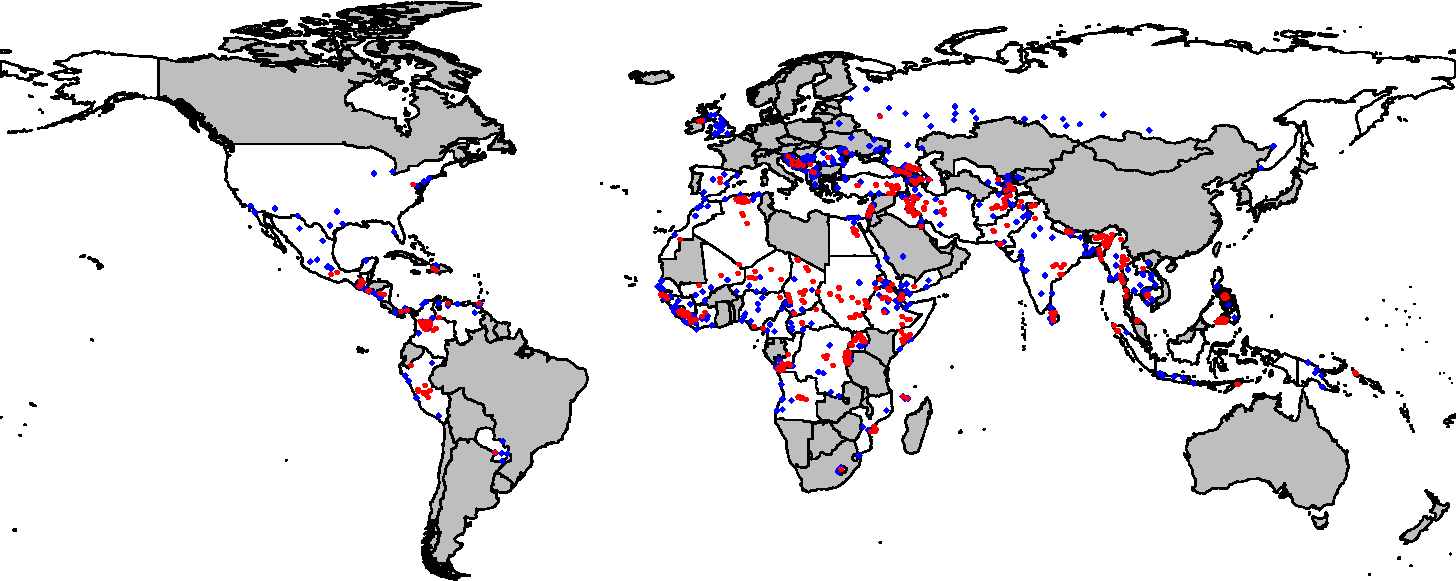
\includegraphics[width=1\textwidth]{CityConfMap-crop}
\end{figure}

\end{frame}
%%%%%%%%%%%%%%%%%%%%%%%%%%%%%%%%%%%%%%%%%

\begin{frame}
\frametitle{Aggregating to Country-Year}

\begin{figure}[ht]
	\centering
	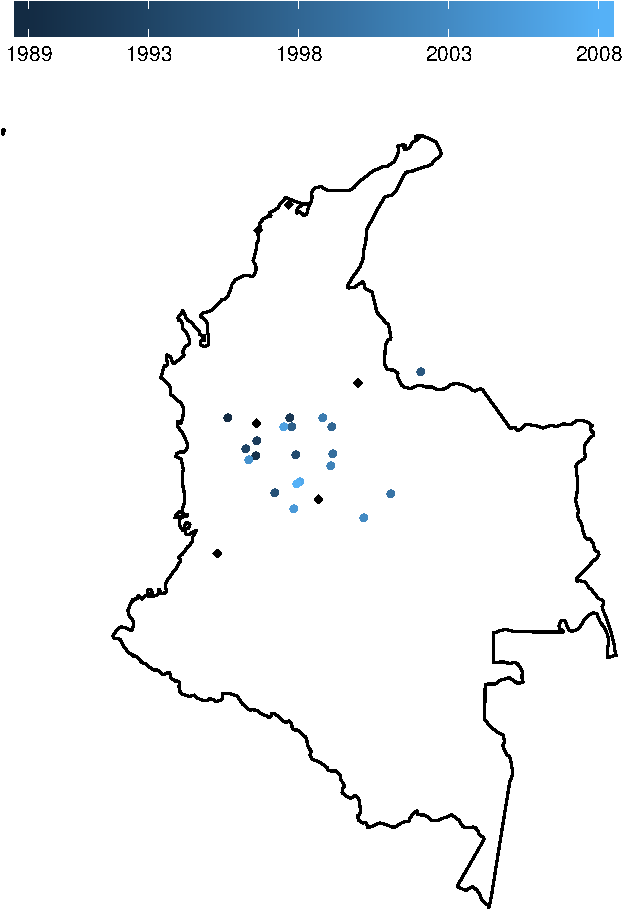
\includegraphics[width=.6\textwidth]{colombiaMap-crop}
\end{figure}

\end{frame}

%%%%%%%%%%%%%%%%%%%%%%%%%%%%%%%%%%%%%%%%%
\begin{frame}
\frametitle{Estimation Approach}

\begin{align*}
	\% \Delta GDP_{i,t} &= \beta_{1}(Upper \; Income_{i,t}) \\
	& \;+\; \beta_{2}(Conflict \; Intensity_{i,t}) \;+\; \beta_{3}(Ln(Conflict \; Area)_{i,t}) \\
	& \;+\; \beta_{4}(Ln(Min. \; Conflict \; Dist.)_{i,t}) \;+\; \beta_{5}(Conflict \; Type_{i,t}) \\
	& \;+\; \beta_{6}(Conflict \; Duration_{i,t}) \;+\; \beta_{7}(Inflation_{i,t-1}) \\
	& \;+\; \beta_{8}(Ln(Land \; Area)_{i,t}) \;+\; \alpha_{i} + \gamma_{t} + \mu_{i,t}
\end{align*}

\end{frame}
%%%%%%%%%%%%%%%%%%%%%%%%%%%%%%%%%%%%%%%%%

%%%%%%%%%%%%%%%%%%%%%%%%%%%%%%%%%%%%%%%%%
\begin{frame}
\frametitle{Findings}

\begin{figure}[ht]
	\centering
	\resizebox{.8\textwidth}{!}{% Created by tikzDevice version 0.6.2 on 2014-03-28 11:43:10
% !TEX encoding = UTF-8 Unicode
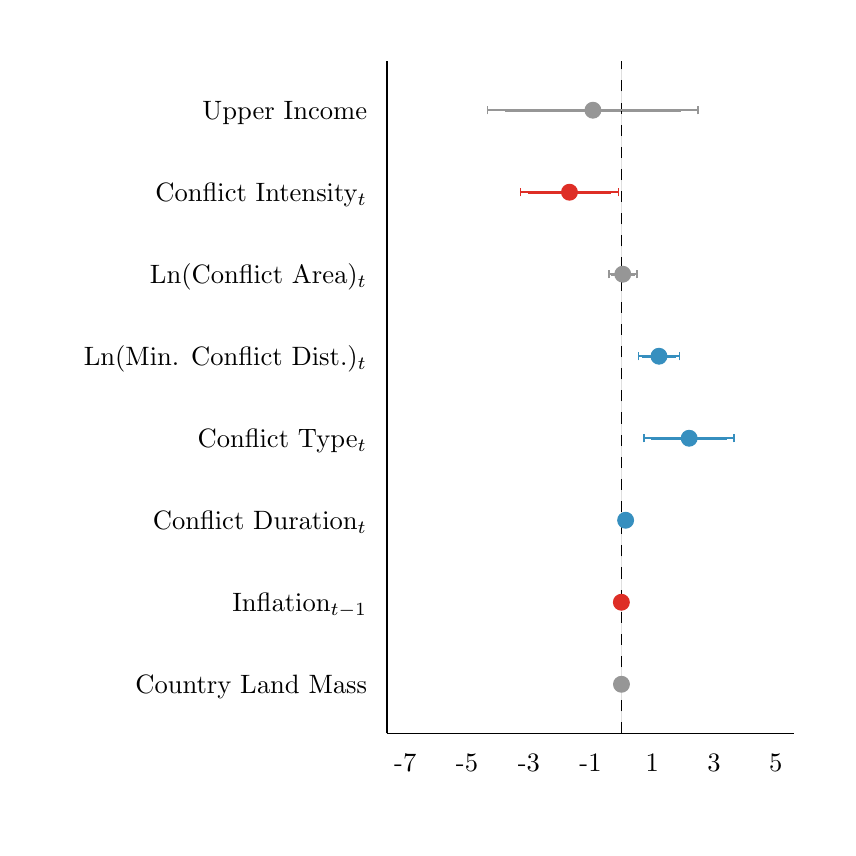
\begin{tikzpicture}[x=1pt,y=1pt]
\definecolor[named]{drawColor}{rgb}{0.00,0.00,0.00}
\definecolor[named]{fillColor}{rgb}{1.00,1.00,1.00}
\fill[color=fillColor,fill opacity=0.00,] (0,0) rectangle (289.08,289.08);
\begin{scope}
\path[clip] (  0.00,  0.00) rectangle (289.08,289.08);
\end{scope}
\begin{scope}
\path[clip] (  0.00,  0.00) rectangle (289.08,289.08);
\end{scope}
\begin{scope}
\path[clip] (  0.00,  0.00) rectangle (289.08,289.08);
\definecolor[named]{drawColor}{rgb}{1.00,1.00,1.00}
\definecolor[named]{fillColor}{rgb}{1.00,1.00,1.00}

\draw[color=drawColor,line width= 0.6pt,line cap=round,line join=round,fill=fillColor,] ( -0.00,  0.00) rectangle (289.08,289.08);
\end{scope}
\begin{scope}
\path[clip] (  0.00,  0.00) rectangle (289.08,289.08);
\end{scope}
\begin{scope}
\path[clip] (  0.00,  0.00) rectangle (289.08,289.08);
\end{scope}
\begin{scope}
\path[clip] (  0.00,  0.00) rectangle (289.08,289.08);
\end{scope}
\begin{scope}
\path[clip] (129.77, 34.03) rectangle (277.03,277.03);
\definecolor[named]{fillColor}{rgb}{1.00,1.00,1.00}

\draw[fill=fillColor,draw opacity=0.00,] (129.77, 34.03) rectangle (277.03,277.03);
\definecolor[named]{drawColor}{rgb}{0.59,0.59,0.59}
\definecolor[named]{fillColor}{rgb}{0.59,0.59,0.59}

\draw[color=drawColor,line width= 0.3pt,line join=round,fill=fillColor,fill opacity=0.30,draw opacity=0.30,] (214.56, 51.82) -- (214.56, 51.82);
\definecolor[named]{drawColor}{rgb}{0.87,0.18,0.15}
\definecolor[named]{fillColor}{rgb}{0.87,0.18,0.15}

\draw[color=drawColor,line width= 0.3pt,line join=round,fill=fillColor,fill opacity=0.30,draw opacity=0.30,] (214.52, 81.45) -- (214.54, 81.45);
\definecolor[named]{drawColor}{rgb}{0.21,0.56,0.75}
\definecolor[named]{fillColor}{rgb}{0.21,0.56,0.75}

\draw[color=drawColor,line width= 0.3pt,line join=round,fill=fillColor,fill opacity=0.30,draw opacity=0.30,] (215.47,111.08) -- (216.65,111.08);

\draw[color=drawColor,line width= 0.3pt,line join=round,fill=fillColor,fill opacity=0.30,draw opacity=0.30,] (222.76,140.72) -- (255.30,140.72);

\draw[color=drawColor,line width= 0.3pt,line join=round,fill=fillColor,fill opacity=0.30,draw opacity=0.30,] (220.66,170.35) -- (235.55,170.35);
\definecolor[named]{drawColor}{rgb}{0.59,0.59,0.59}
\definecolor[named]{fillColor}{rgb}{0.59,0.59,0.59}

\draw[color=drawColor,line width= 0.3pt,line join=round,fill=fillColor,fill opacity=0.30,draw opacity=0.30,] (209.97,199.99) -- (220.09,199.99);
\definecolor[named]{drawColor}{rgb}{0.87,0.18,0.15}
\definecolor[named]{fillColor}{rgb}{0.87,0.18,0.15}

\draw[color=drawColor,line width= 0.3pt,line join=round,fill=fillColor,fill opacity=0.30,draw opacity=0.30,] (178.06,229.62) -- (213.50,229.62);
\definecolor[named]{drawColor}{rgb}{0.59,0.59,0.59}
\definecolor[named]{fillColor}{rgb}{0.59,0.59,0.59}

\draw[color=drawColor,line width= 0.3pt,line join=round,fill=fillColor,fill opacity=0.30,draw opacity=0.30,] (166.20,259.25) -- (242.30,259.25);
\definecolor[named]{drawColor}{rgb}{0.59,0.59,0.59}
\definecolor[named]{fillColor}{rgb}{0.59,0.59,0.59}

\draw[color=drawColor,line width= 1.1pt,line join=round,fill=fillColor,] (214.56, 51.82) -- (214.56, 51.82);
\definecolor[named]{drawColor}{rgb}{0.87,0.18,0.15}
\definecolor[named]{fillColor}{rgb}{0.87,0.18,0.15}

\draw[color=drawColor,line width= 1.1pt,line join=round,fill=fillColor,] (214.52, 81.45) -- (214.53, 81.45);
\definecolor[named]{drawColor}{rgb}{0.21,0.56,0.75}
\definecolor[named]{fillColor}{rgb}{0.21,0.56,0.75}

\draw[color=drawColor,line width= 1.1pt,line join=round,fill=fillColor,] (215.57,111.08) -- (216.56,111.08);

\draw[color=drawColor,line width= 1.1pt,line join=round,fill=fillColor,] (225.38,140.72) -- (252.69,140.72);

\draw[color=drawColor,line width= 1.1pt,line join=round,fill=fillColor,] (221.86,170.35) -- (234.36,170.35);
\definecolor[named]{drawColor}{rgb}{0.59,0.59,0.59}
\definecolor[named]{fillColor}{rgb}{0.59,0.59,0.59}

\draw[color=drawColor,line width= 1.1pt,line join=round,fill=fillColor,] (210.79,199.99) -- (219.28,199.99);
\definecolor[named]{drawColor}{rgb}{0.87,0.18,0.15}
\definecolor[named]{fillColor}{rgb}{0.87,0.18,0.15}

\draw[color=drawColor,line width= 1.1pt,line join=round,fill=fillColor,] (180.91,229.62) -- (210.65,229.62);
\definecolor[named]{drawColor}{rgb}{0.59,0.59,0.59}
\definecolor[named]{fillColor}{rgb}{0.59,0.59,0.59}

\draw[color=drawColor,line width= 1.1pt,line join=round,fill=fillColor,] (172.32,259.25) -- (236.19,259.25);
\definecolor[named]{drawColor}{rgb}{0.00,0.00,0.00}
\definecolor[named]{fillColor}{rgb}{0.00,0.00,0.00}

\draw[color=drawColor,line width= 0.6pt,dash pattern=on 4pt off 4pt ,line join=round,fill=fillColor,] (214.56, 34.03) -- (214.56,277.03);
\definecolor[named]{drawColor}{rgb}{0.59,0.59,0.59}
\definecolor[named]{fillColor}{rgb}{0.59,0.59,0.59}

\draw[color=drawColor,line cap=round,line join=round,fill=fillColor,] (204.25,259.25) circle (  2.85);
\definecolor[named]{drawColor}{rgb}{0.87,0.18,0.15}
\definecolor[named]{fillColor}{rgb}{0.87,0.18,0.15}

\draw[color=drawColor,line cap=round,line join=round,fill=fillColor,] (195.78,229.62) circle (  2.85);
\definecolor[named]{drawColor}{rgb}{0.59,0.59,0.59}
\definecolor[named]{fillColor}{rgb}{0.59,0.59,0.59}

\draw[color=drawColor,line cap=round,line join=round,fill=fillColor,] (215.03,199.99) circle (  2.85);
\definecolor[named]{drawColor}{rgb}{0.21,0.56,0.75}
\definecolor[named]{fillColor}{rgb}{0.21,0.56,0.75}

\draw[color=drawColor,line cap=round,line join=round,fill=fillColor,] (228.11,170.35) circle (  2.85);

\draw[color=drawColor,line cap=round,line join=round,fill=fillColor,] (239.03,140.72) circle (  2.85);

\draw[color=drawColor,line cap=round,line join=round,fill=fillColor,] (216.06,111.08) circle (  2.85);
\definecolor[named]{drawColor}{rgb}{0.87,0.18,0.15}
\definecolor[named]{fillColor}{rgb}{0.87,0.18,0.15}

\draw[color=drawColor,line cap=round,line join=round,fill=fillColor,] (214.53, 81.45) circle (  2.85);
\definecolor[named]{drawColor}{rgb}{0.59,0.59,0.59}
\definecolor[named]{fillColor}{rgb}{0.59,0.59,0.59}

\draw[color=drawColor,line cap=round,line join=round,fill=fillColor,] (214.56, 51.82) circle (  2.85);

\draw[color=drawColor,line width= 0.6pt,line join=round,] (214.56, 50.33) --
	(214.56, 53.30);

\draw[color=drawColor,line width= 0.6pt,line join=round,] (214.56, 51.82) --
	(214.56, 51.82);

\draw[color=drawColor,line width= 0.6pt,line join=round,] (214.56, 50.33) --
	(214.56, 53.30);
\definecolor[named]{drawColor}{rgb}{0.87,0.18,0.15}
\definecolor[named]{fillColor}{rgb}{0.87,0.18,0.15}

\draw[color=drawColor,line width= 0.6pt,line join=round,] (214.54, 79.97) --
	(214.54, 82.93);

\draw[color=drawColor,line width= 0.6pt,line join=round,] (214.54, 81.45) --
	(214.52, 81.45);

\draw[color=drawColor,line width= 0.6pt,line join=round,] (214.52, 79.97) --
	(214.52, 82.93);
\definecolor[named]{drawColor}{rgb}{0.21,0.56,0.75}
\definecolor[named]{fillColor}{rgb}{0.21,0.56,0.75}

\draw[color=drawColor,line width= 0.6pt,line join=round,] (216.65,109.60) --
	(216.65,112.57);

\draw[color=drawColor,line width= 0.6pt,line join=round,] (216.65,111.08) --
	(215.47,111.08);

\draw[color=drawColor,line width= 0.6pt,line join=round,] (215.47,109.60) --
	(215.47,112.57);

\draw[color=drawColor,line width= 0.6pt,line join=round,] (255.30,139.24) --
	(255.30,142.20);

\draw[color=drawColor,line width= 0.6pt,line join=round,] (255.30,140.72) --
	(222.76,140.72);

\draw[color=drawColor,line width= 0.6pt,line join=round,] (222.76,139.24) --
	(222.76,142.20);

\draw[color=drawColor,line width= 0.6pt,line join=round,] (235.55,168.87) --
	(235.55,171.83);

\draw[color=drawColor,line width= 0.6pt,line join=round,] (235.55,170.35) --
	(220.66,170.35);

\draw[color=drawColor,line width= 0.6pt,line join=round,] (220.66,168.87) --
	(220.66,171.83);
\definecolor[named]{drawColor}{rgb}{0.59,0.59,0.59}
\definecolor[named]{fillColor}{rgb}{0.59,0.59,0.59}

\draw[color=drawColor,line width= 0.6pt,line join=round,] (220.09,198.50) --
	(220.09,201.47);

\draw[color=drawColor,line width= 0.6pt,line join=round,] (220.09,199.99) --
	(209.97,199.99);

\draw[color=drawColor,line width= 0.6pt,line join=round,] (209.97,198.50) --
	(209.97,201.47);
\definecolor[named]{drawColor}{rgb}{0.87,0.18,0.15}
\definecolor[named]{fillColor}{rgb}{0.87,0.18,0.15}

\draw[color=drawColor,line width= 0.6pt,line join=round,] (213.50,228.14) --
	(213.50,231.10);

\draw[color=drawColor,line width= 0.6pt,line join=round,] (213.50,229.62) --
	(178.06,229.62);

\draw[color=drawColor,line width= 0.6pt,line join=round,] (178.06,228.14) --
	(178.06,231.10);
\definecolor[named]{drawColor}{rgb}{0.59,0.59,0.59}
\definecolor[named]{fillColor}{rgb}{0.59,0.59,0.59}

\draw[color=drawColor,line width= 0.6pt,line join=round,] (242.30,257.77) --
	(242.30,260.74);

\draw[color=drawColor,line width= 0.6pt,line join=round,] (242.30,259.25) --
	(166.20,259.25);

\draw[color=drawColor,line width= 0.6pt,line join=round,] (166.20,257.77) --
	(166.20,260.74);
\end{scope}
\begin{scope}
\path[clip] (  0.00,  0.00) rectangle (289.08,289.08);
\end{scope}
\begin{scope}
\path[clip] (  0.00,  0.00) rectangle (289.08,289.08);
\definecolor[named]{drawColor}{rgb}{0.00,0.00,0.00}

\draw[color=drawColor,line width= 0.6pt,line join=round,fill opacity=0.00,] (129.77, 34.03) --
	(129.77,277.03);
\end{scope}
\begin{scope}
\path[clip] (  0.00,  0.00) rectangle (289.08,289.08);
\definecolor[named]{drawColor}{rgb}{0.00,0.00,0.00}

\node[color=drawColor,anchor=base east,inner sep=0pt, outer sep=0pt, scale=  0.96] at (122.65, 48.51) {Country Land Mass};

\node[color=drawColor,anchor=base east,inner sep=0pt, outer sep=0pt, scale=  0.96] at (122.65, 78.14) {Inflation$_{t-1}$};

\node[color=drawColor,anchor=base east,inner sep=0pt, outer sep=0pt, scale=  0.96] at (122.65,107.78) {Conflict Duration$_{t}$};

\node[color=drawColor,anchor=base east,inner sep=0pt, outer sep=0pt, scale=  0.96] at (122.65,137.41) {Conflict Type$_{t}$};

\node[color=drawColor,anchor=base east,inner sep=0pt, outer sep=0pt, scale=  0.96] at (122.65,167.05) {Ln(Min. Conflict Dist.)$_{t}$};

\node[color=drawColor,anchor=base east,inner sep=0pt, outer sep=0pt, scale=  0.96] at (122.65,196.68) {Ln(Conflict Area)$_{t}$};

\node[color=drawColor,anchor=base east,inner sep=0pt, outer sep=0pt, scale=  0.96] at (122.65,226.31) {Conflict Intensity$_{t}$};

\node[color=drawColor,anchor=base east,inner sep=0pt, outer sep=0pt, scale=  0.96] at (122.65,255.95) {Upper Income};
\end{scope}
\begin{scope}
\path[clip] (  0.00,  0.00) rectangle (289.08,289.08);
\end{scope}
\begin{scope}
\path[clip] (  0.00,  0.00) rectangle (289.08,289.08);
\end{scope}
\begin{scope}
\path[clip] (  0.00,  0.00) rectangle (289.08,289.08);
\end{scope}
\begin{scope}
\path[clip] (  0.00,  0.00) rectangle (289.08,289.08);
\end{scope}
\begin{scope}
\path[clip] (  0.00,  0.00) rectangle (289.08,289.08);
\end{scope}
\begin{scope}
\path[clip] (  0.00,  0.00) rectangle (289.08,289.08);
\end{scope}
\begin{scope}
\path[clip] (  0.00,  0.00) rectangle (289.08,289.08);
\definecolor[named]{drawColor}{rgb}{0.00,0.00,0.00}

\draw[color=drawColor,line width= 0.6pt,line join=round,fill opacity=0.00,] (129.77, 34.03) --
	(277.03, 34.03);
\end{scope}
\begin{scope}
\path[clip] (  0.00,  0.00) rectangle (289.08,289.08);
\end{scope}
\begin{scope}
\path[clip] (  0.00,  0.00) rectangle (289.08,289.08);
\end{scope}
\begin{scope}
\path[clip] (  0.00,  0.00) rectangle (289.08,289.08);
\definecolor[named]{drawColor}{rgb}{0.00,0.00,0.00}

\node[color=drawColor,anchor=base,inner sep=0pt, outer sep=0pt, scale=  0.96] at (136.46, 20.31) {-7};

\node[color=drawColor,anchor=base,inner sep=0pt, outer sep=0pt, scale=  0.96] at (158.77, 20.31) {-5};

\node[color=drawColor,anchor=base,inner sep=0pt, outer sep=0pt, scale=  0.96] at (181.09, 20.31) {-3};

\node[color=drawColor,anchor=base,inner sep=0pt, outer sep=0pt, scale=  0.96] at (203.40, 20.31) {-1};

\node[color=drawColor,anchor=base,inner sep=0pt, outer sep=0pt, scale=  0.96] at (225.71, 20.31) {1};

\node[color=drawColor,anchor=base,inner sep=0pt, outer sep=0pt, scale=  0.96] at (248.03, 20.31) {3};

\node[color=drawColor,anchor=base,inner sep=0pt, outer sep=0pt, scale=  0.96] at (270.34, 20.31) {5};
\end{scope}
\begin{scope}
\path[clip] (  0.00,  0.00) rectangle (289.08,289.08);
\end{scope}
\begin{scope}
\path[clip] (  0.00,  0.00) rectangle (289.08,289.08);
\end{scope}
\begin{scope}
\path[clip] (  0.00,  0.00) rectangle (289.08,289.08);
\end{scope}
\begin{scope}
\path[clip] (  0.00,  0.00) rectangle (289.08,289.08);
\end{scope}
\begin{scope}
\path[clip] (  0.00,  0.00) rectangle (289.08,289.08);
\end{scope}
\begin{scope}
\path[clip] (  0.00,  0.00) rectangle (289.08,289.08);
\end{scope}
\begin{scope}
\path[clip] (  0.00,  0.00) rectangle (289.08,289.08);
\end{scope}
\begin{scope}
\path[clip] (  0.00,  0.00) rectangle (289.08,289.08);
\end{scope}
\begin{scope}
\path[clip] (  0.00,  0.00) rectangle (289.08,289.08);
\end{scope}
\begin{scope}
\path[clip] (  0.00,  0.00) rectangle (289.08,289.08);
\end{scope}
\begin{scope}
\path[clip] (  0.00,  0.00) rectangle (289.08,289.08);
\end{scope}
\end{tikzpicture}
}
\end{figure}

\end{frame}
%%%%%%%%%%%%%%%%%%%%%%%%%%%%%%%%%%%%%%%%%

\begin{frame}
\frametitle{Substantive Effects}

\begin{figure}[ht]
	\centering
	\resizebox{.9\textwidth}{!}{% Created by tikzDevice version 0.6.2 on 2014-03-28 19:46:55
% !TEX encoding = UTF-8 Unicode
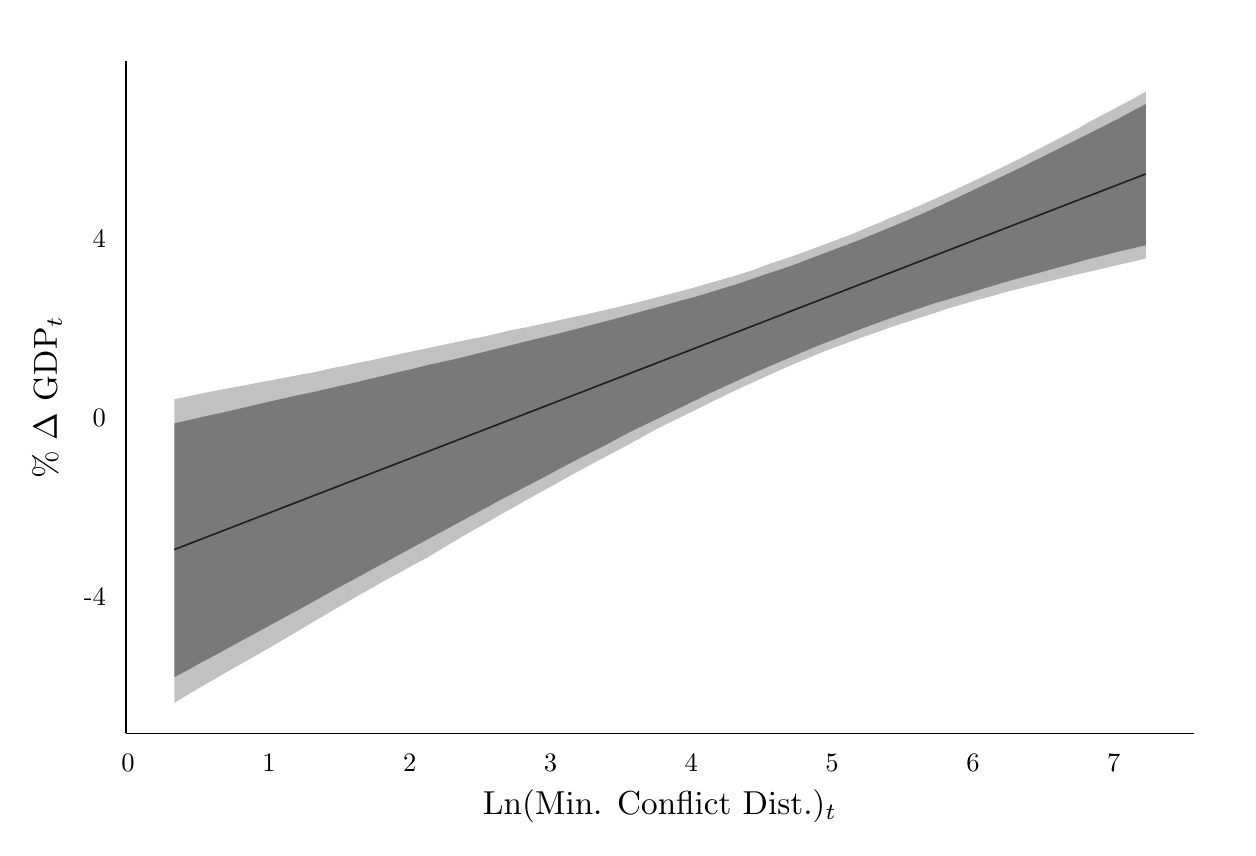
\begin{tikzpicture}[x=1pt,y=1pt]
\definecolor[named]{drawColor}{rgb}{0.00,0.00,0.00}
\definecolor[named]{fillColor}{rgb}{1.00,1.00,1.00}
\fill[color=fillColor,fill opacity=0.00,] (0,0) rectangle (433.62,289.08);
\begin{scope}
\path[clip] (  0.00,  0.00) rectangle (433.62,289.08);
\end{scope}
\begin{scope}
\path[clip] (  0.00,  0.00) rectangle (433.62,289.08);
\end{scope}
\begin{scope}
\path[clip] (  0.00,  0.00) rectangle (433.62,289.08);
\definecolor[named]{drawColor}{rgb}{1.00,1.00,1.00}
\definecolor[named]{fillColor}{rgb}{1.00,1.00,1.00}

\draw[color=drawColor,line width= 0.6pt,line cap=round,line join=round,fill=fillColor,] (  0.00,  0.00) rectangle (433.62,289.08);
\end{scope}
\begin{scope}
\path[clip] (  0.00,  0.00) rectangle (433.62,289.08);
\end{scope}
\begin{scope}
\path[clip] (  0.00,  0.00) rectangle (433.62,289.08);
\end{scope}
\begin{scope}
\path[clip] (  0.00,  0.00) rectangle (433.62,289.08);
\end{scope}
\begin{scope}
\path[clip] ( 35.42, 34.03) rectangle (421.57,277.03);
\definecolor[named]{fillColor}{rgb}{1.00,1.00,1.00}

\draw[fill=fillColor,draw opacity=0.00,] ( 35.42, 34.03) rectangle (421.57,277.03);
\definecolor[named]{drawColor}{rgb}{0.00,0.00,0.00}
\definecolor[named]{fillColor}{rgb}{0.00,0.00,0.00}

\draw[color=drawColor,line width= 0.6pt,line join=round,] ( 52.97,100.48) --
	( 58.06,102.45) --
	( 63.15,104.42) --
	( 68.24,106.39) --
	( 73.32,108.35) --
	( 78.41,110.32) --
	( 83.50,112.29) --
	( 88.59,114.25) --
	( 93.67,116.22) --
	( 98.76,118.19) --
	(103.85,120.16) --
	(108.94,122.12) --
	(114.03,124.09) --
	(119.11,126.06) --
	(124.20,128.02) --
	(129.29,129.99) --
	(134.38,131.96) --
	(139.46,133.93) --
	(144.55,135.89) --
	(149.64,137.86) --
	(154.73,139.83) --
	(159.81,141.80) --
	(164.90,143.76) --
	(169.99,145.73) --
	(175.08,147.70) --
	(180.17,149.66) --
	(185.25,151.63) --
	(190.34,153.60) --
	(195.43,155.57) --
	(200.52,157.53) --
	(205.60,159.50) --
	(210.69,161.47) --
	(215.78,163.43) --
	(220.87,165.40) --
	(225.95,167.37) --
	(231.04,169.34) --
	(236.13,171.30) --
	(241.22,173.27) --
	(246.30,175.24) --
	(251.39,177.20) --
	(256.48,179.17) --
	(261.57,181.14) --
	(266.66,183.11) --
	(271.74,185.07) --
	(276.83,187.04) --
	(281.92,189.01) --
	(287.01,190.98) --
	(292.09,192.94) --
	(297.18,194.91) --
	(302.27,196.88) --
	(307.36,198.84) --
	(312.44,200.81) --
	(317.53,202.78) --
	(322.62,204.75) --
	(327.71,206.71) --
	(332.80,208.68) --
	(337.88,210.65) --
	(342.97,212.61) --
	(348.06,214.58) --
	(353.15,216.55) --
	(358.23,218.52) --
	(363.32,220.48) --
	(368.41,222.45) --
	(373.50,224.42) --
	(378.58,226.39) --
	(383.67,228.35) --
	(388.76,230.32) --
	(393.85,232.29) --
	(398.93,234.25) --
	(404.02,236.22);
\definecolor[named]{fillColor}{rgb}{0.20,0.20,0.20}

\draw[fill=fillColor,fill opacity=0.30,draw opacity=0.00,] ( 52.97,154.81) --
	( 58.06,155.84) --
	( 63.15,156.96) --
	( 68.24,157.95) --
	( 73.32,158.93) --
	( 78.41,159.86) --
	( 83.50,160.85) --
	( 88.59,161.77) --
	( 93.67,162.75) --
	( 98.76,163.72) --
	(103.85,164.62) --
	(108.94,165.84) --
	(114.03,166.82) --
	(119.11,167.92) --
	(124.20,168.91) --
	(129.29,170.03) --
	(134.38,171.13) --
	(139.46,172.18) --
	(144.55,173.24) --
	(149.64,174.34) --
	(154.73,175.44) --
	(159.81,176.47) --
	(164.90,177.47) --
	(169.99,178.63) --
	(175.08,179.85) --
	(180.17,180.81) --
	(185.25,181.91) --
	(190.34,182.95) --
	(195.43,184.18) --
	(200.52,185.19) --
	(205.60,186.36) --
	(210.69,187.52) --
	(215.78,188.72) --
	(220.87,189.93) --
	(225.95,191.25) --
	(231.04,192.59) --
	(236.13,193.91) --
	(241.22,195.29) --
	(246.30,196.77) --
	(251.39,198.21) --
	(256.48,199.69) --
	(261.57,201.30) --
	(266.66,203.24) --
	(271.74,204.95) --
	(276.83,206.66) --
	(281.92,208.49) --
	(287.01,210.37) --
	(292.09,212.31) --
	(297.18,214.17) --
	(302.27,216.35) --
	(307.36,218.44) --
	(312.44,220.66) --
	(317.53,222.74) --
	(322.62,224.90) --
	(327.71,227.17) --
	(332.80,229.46) --
	(337.88,231.80) --
	(342.97,234.23) --
	(348.06,236.60) --
	(353.15,239.13) --
	(358.23,241.60) --
	(363.32,244.22) --
	(368.41,246.82) --
	(373.50,249.48) --
	(378.58,252.11) --
	(383.67,255.07) --
	(388.76,257.75) --
	(393.85,260.38) --
	(398.93,263.07) --
	(404.02,265.99) --
	(404.02,205.70) --
	(398.93,204.43) --
	(393.85,203.35) --
	(388.76,202.08) --
	(383.67,200.93) --
	(378.58,199.75) --
	(373.50,198.52) --
	(368.41,197.29) --
	(363.32,196.01) --
	(358.23,194.78) --
	(353.15,193.45) --
	(348.06,192.00) --
	(342.97,190.65) --
	(337.88,189.13) --
	(332.80,187.67) --
	(327.71,185.97) --
	(322.62,184.33) --
	(317.53,182.67) --
	(312.44,181.05) --
	(307.36,179.19) --
	(302.27,177.46) --
	(297.18,175.59) --
	(292.09,173.73) --
	(287.01,171.79) --
	(281.92,169.67) --
	(276.83,167.52) --
	(271.74,165.30) --
	(266.66,163.01) --
	(261.57,160.68) --
	(256.48,158.37) --
	(251.39,155.95) --
	(246.30,153.44) --
	(241.22,150.92) --
	(236.13,148.38) --
	(231.04,145.95) --
	(225.95,143.32) --
	(220.87,140.49) --
	(215.78,137.71) --
	(210.69,135.03) --
	(205.60,132.36) --
	(200.52,129.60) --
	(195.43,126.84) --
	(190.34,123.95) --
	(185.25,121.21) --
	(180.17,118.35) --
	(175.08,115.46) --
	(169.99,112.63) --
	(164.90,109.64) --
	(159.81,106.78) --
	(154.73,103.82) --
	(149.64,100.79) --
	(144.55, 97.69) --
	(139.46, 94.99) --
	(134.38, 92.15) --
	(129.29, 89.41) --
	(124.20, 86.56) --
	(119.11, 83.67) --
	(114.03, 80.71) --
	(108.94, 77.74) --
	(103.85, 74.75) --
	( 98.76, 71.73) --
	( 93.67, 68.73) --
	( 88.59, 65.72) --
	( 83.50, 62.81) --
	( 78.41, 59.88) --
	( 73.32, 57.06) --
	( 68.24, 54.11) --
	( 63.15, 51.16) --
	( 58.06, 48.18) --
	( 52.97, 45.08) --
	cycle;
\definecolor[named]{fillColor}{rgb}{0.20,0.20,0.20}

\draw[fill=fillColor,fill opacity=0.50,draw opacity=0.00,] ( 52.97,146.09) --
	( 58.06,147.23) --
	( 63.15,148.43) --
	( 68.24,149.52) --
	( 73.32,150.65) --
	( 78.41,151.86) --
	( 83.50,153.05) --
	( 88.59,154.24) --
	( 93.67,155.36) --
	( 98.76,156.50) --
	(103.85,157.53) --
	(108.94,158.74) --
	(114.03,159.89) --
	(119.11,161.03) --
	(124.20,162.30) --
	(129.29,163.46) --
	(134.38,164.71) --
	(139.46,165.87) --
	(144.55,167.17) --
	(149.64,168.28) --
	(154.73,169.39) --
	(159.81,170.65) --
	(164.90,171.93) --
	(169.99,173.18) --
	(175.08,174.45) --
	(180.17,175.74) --
	(185.25,176.95) --
	(190.34,178.19) --
	(195.43,179.45) --
	(200.52,180.81) --
	(205.60,182.12) --
	(210.69,183.47) --
	(215.78,184.85) --
	(220.87,186.25) --
	(225.95,187.63) --
	(231.04,189.04) --
	(236.13,190.51) --
	(241.22,191.82) --
	(246.30,193.35) --
	(251.39,194.93) --
	(256.48,196.49) --
	(261.57,198.21) --
	(266.66,199.97) --
	(271.74,201.61) --
	(276.83,203.37) --
	(281.92,205.30) --
	(287.01,207.25) --
	(292.09,209.16) --
	(297.18,211.07) --
	(302.27,213.04) --
	(307.36,215.14) --
	(312.44,217.21) --
	(317.53,219.36) --
	(322.62,221.56) --
	(327.71,223.87) --
	(332.80,226.21) --
	(337.88,228.58) --
	(342.97,231.00) --
	(348.06,233.40) --
	(353.15,235.83) --
	(358.23,238.21) --
	(363.32,240.77) --
	(368.41,243.25) --
	(373.50,245.81) --
	(378.58,248.32) --
	(383.67,250.89) --
	(388.76,253.46) --
	(393.85,256.04) --
	(398.93,258.80) --
	(404.02,261.46) --
	(404.02,210.45) --
	(398.93,209.26) --
	(393.85,208.09) --
	(388.76,206.80) --
	(383.67,205.52) --
	(378.58,204.09) --
	(373.50,202.73) --
	(368.41,201.33) --
	(363.32,199.93) --
	(358.23,198.58) --
	(353.15,197.10) --
	(348.06,195.62) --
	(342.97,194.05) --
	(337.88,192.49) --
	(332.80,190.98) --
	(327.71,189.50) --
	(322.62,187.79) --
	(317.53,186.08) --
	(312.44,184.36) --
	(307.36,182.50) --
	(302.27,180.65) --
	(297.18,178.67) --
	(292.09,176.69) --
	(287.01,174.75) --
	(281.92,172.67) --
	(276.83,170.47) --
	(271.74,168.31) --
	(266.66,166.16) --
	(261.57,163.88) --
	(256.48,161.55) --
	(251.39,159.21) --
	(246.30,156.88) --
	(241.22,154.39) --
	(236.13,151.93) --
	(231.04,149.46) --
	(225.95,146.97) --
	(220.87,144.56) --
	(215.78,142.02) --
	(210.69,139.24) --
	(205.60,136.61) --
	(200.52,134.04) --
	(195.43,131.41) --
	(190.34,128.69) --
	(185.25,125.94) --
	(180.17,123.36) --
	(175.08,120.64) --
	(169.99,117.98) --
	(164.90,115.19) --
	(159.81,112.46) --
	(154.73,109.70) --
	(149.64,106.93) --
	(144.55,104.24) --
	(139.46,101.46) --
	(134.38, 98.69) --
	(129.29, 95.92) --
	(124.20, 93.22) --
	(119.11, 90.39) --
	(114.03, 87.67) --
	(108.94, 84.91) --
	(103.85, 82.04) --
	( 98.76, 79.21) --
	( 93.67, 76.46) --
	( 88.59, 73.69) --
	( 83.50, 70.90) --
	( 78.41, 68.17) --
	( 73.32, 65.41) --
	( 68.24, 62.58) --
	( 63.15, 59.92) --
	( 58.06, 57.06) --
	( 52.97, 54.35) --
	cycle;
\end{scope}
\begin{scope}
\path[clip] (  0.00,  0.00) rectangle (433.62,289.08);
\end{scope}
\begin{scope}
\path[clip] (  0.00,  0.00) rectangle (433.62,289.08);
\definecolor[named]{drawColor}{rgb}{0.00,0.00,0.00}

\draw[color=drawColor,line width= 0.6pt,line join=round,fill opacity=0.00,] ( 35.42, 34.03) --
	( 35.42,277.03);
\end{scope}
\begin{scope}
\path[clip] (  0.00,  0.00) rectangle (433.62,289.08);
\definecolor[named]{drawColor}{rgb}{0.00,0.00,0.00}

\node[color=drawColor,anchor=base east,inner sep=0pt, outer sep=0pt, scale=  0.96] at ( 28.31, 80.40) {-4};

\node[color=drawColor,anchor=base east,inner sep=0pt, outer sep=0pt, scale=  0.96] at ( 28.31,145.11) {0};

\node[color=drawColor,anchor=base east,inner sep=0pt, outer sep=0pt, scale=  0.96] at ( 28.31,209.82) {4};
\end{scope}
\begin{scope}
\path[clip] (  0.00,  0.00) rectangle (433.62,289.08);
\end{scope}
\begin{scope}
\path[clip] (  0.00,  0.00) rectangle (433.62,289.08);
\end{scope}
\begin{scope}
\path[clip] (  0.00,  0.00) rectangle (433.62,289.08);
\end{scope}
\begin{scope}
\path[clip] (  0.00,  0.00) rectangle (433.62,289.08);
\end{scope}
\begin{scope}
\path[clip] (  0.00,  0.00) rectangle (433.62,289.08);
\end{scope}
\begin{scope}
\path[clip] (  0.00,  0.00) rectangle (433.62,289.08);
\end{scope}
\begin{scope}
\path[clip] (  0.00,  0.00) rectangle (433.62,289.08);
\definecolor[named]{drawColor}{rgb}{0.00,0.00,0.00}

\draw[color=drawColor,line width= 0.6pt,line join=round,fill opacity=0.00,] ( 35.42, 34.03) --
	(421.57, 34.03);
\end{scope}
\begin{scope}
\path[clip] (  0.00,  0.00) rectangle (433.62,289.08);
\end{scope}
\begin{scope}
\path[clip] (  0.00,  0.00) rectangle (433.62,289.08);
\end{scope}
\begin{scope}
\path[clip] (  0.00,  0.00) rectangle (433.62,289.08);
\definecolor[named]{drawColor}{rgb}{0.00,0.00,0.00}

\node[color=drawColor,anchor=base,inner sep=0pt, outer sep=0pt, scale=  0.96] at ( 36.30, 20.31) {0};

\node[color=drawColor,anchor=base,inner sep=0pt, outer sep=0pt, scale=  0.96] at ( 87.18, 20.31) {1};

\node[color=drawColor,anchor=base,inner sep=0pt, outer sep=0pt, scale=  0.96] at (138.05, 20.31) {2};

\node[color=drawColor,anchor=base,inner sep=0pt, outer sep=0pt, scale=  0.96] at (188.93, 20.31) {3};

\node[color=drawColor,anchor=base,inner sep=0pt, outer sep=0pt, scale=  0.96] at (239.81, 20.31) {4};

\node[color=drawColor,anchor=base,inner sep=0pt, outer sep=0pt, scale=  0.96] at (290.68, 20.31) {5};

\node[color=drawColor,anchor=base,inner sep=0pt, outer sep=0pt, scale=  0.96] at (341.56, 20.31) {6};

\node[color=drawColor,anchor=base,inner sep=0pt, outer sep=0pt, scale=  0.96] at (392.44, 20.31) {7};
\end{scope}
\begin{scope}
\path[clip] (  0.00,  0.00) rectangle (433.62,289.08);
\end{scope}
\begin{scope}
\path[clip] (  0.00,  0.00) rectangle (433.62,289.08);
\end{scope}
\begin{scope}
\path[clip] (  0.00,  0.00) rectangle (433.62,289.08);
\end{scope}
\begin{scope}
\path[clip] (  0.00,  0.00) rectangle (433.62,289.08);
\end{scope}
\begin{scope}
\path[clip] (  0.00,  0.00) rectangle (433.62,289.08);
\definecolor[named]{drawColor}{rgb}{0.00,0.00,0.00}

\node[color=drawColor,anchor=base,inner sep=0pt, outer sep=0pt, scale=  1.20] at (228.50,  4.82) {Ln(Min. Conflict Dist.)$_{t}$};
\end{scope}
\begin{scope}
\path[clip] (  0.00,  0.00) rectangle (433.62,289.08);
\end{scope}
\begin{scope}
\path[clip] (  0.00,  0.00) rectangle (433.62,289.08);
\definecolor[named]{drawColor}{rgb}{0.00,0.00,0.00}

\node[rotate= 90.00,color=drawColor,anchor=base,inner sep=0pt, outer sep=0pt, scale=  1.20] at ( 10.53,155.53) {\% $\Delta$ GDP$_{t}$};
\end{scope}
\begin{scope}
\path[clip] (  0.00,  0.00) rectangle (433.62,289.08);
\end{scope}
\begin{scope}
\path[clip] (  0.00,  0.00) rectangle (433.62,289.08);
\end{scope}
\begin{scope}
\path[clip] (  0.00,  0.00) rectangle (433.62,289.08);
\end{scope}
\begin{scope}
\path[clip] (  0.00,  0.00) rectangle (433.62,289.08);
\end{scope}
\end{tikzpicture}
}
\end{figure}

\end{frame}

%%%%%%%%%%%%%%%%%%%%%%%%%%%%%%%%%%%%%%%%%
\begin{frame}
\frametitle{Conclusions \& Next Steps}

\begin{block}{Conclusions}
\begin{itemize}
	\item Novel approach in the study of civil conflict to distinguish between spatially dissimilar events
	\item Proximity of conflict to major cities explains disparate economic outcomes
\end{itemize}
\end{block}

\begin{block}{Next Steps}
\begin{itemize}
\item Account for other economically important locations (e.g., oil fields)
\item Alternative methods to address aggregation problem
\item More refined analysis within a country using subnational economic data
\end{itemize}
\end{block}

\end{frame}

%%%%%%%%%%%%%%%%%%%%%%%%%%%%%%%%%%%%%%%%%

\plain{Thanks}

\end{document}
